\documentclass[tikz,border=.5em]{standalone}
\usepackage{amssymb}
\usetikzlibrary{positioning,shapes}
\tikzstyle{space} = [
    draw,
    ellipse,
    minimum width=2.8cm,
    minimum height=1.8cm]

\def\X{\mathcal{X}}
\def\H{\mathcal{H}}

\begin{document}
    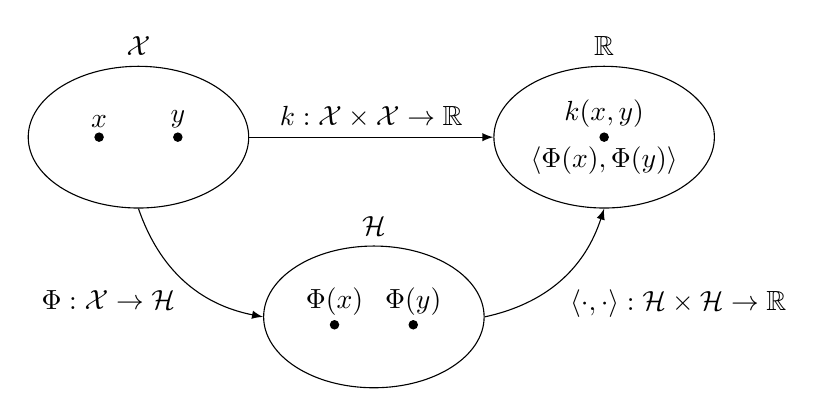
\begin{tikzpicture}
        \node[space] (X) {};
        \draw (X.north) node[above]{\(\X\)};
        \filldraw (X.center) ++(-.5,0) circle(1.5pt) node[above]{\(x\)};
        \filldraw (X.center) ++(.5,0) circle(1.5pt) node[above]{\(y\)};

        \node[space] (F) [below right = and 1cm of X] {};
        \draw (F.north) node[above]{\(\H\)};
        \filldraw (F.center) ++(-.5,-.1) circle(1.5pt) node[above]{\(\Phi(x)\)};
        \filldraw (F.center) ++(.5,-.1) circle(1.5pt) node[above]{\(\Phi(y)\)};

        \node[space] (R) [right = 3.1cm of X] {};
        \draw (R.north) node[above]{\(\mathbb{R}\)};
        \filldraw (R.center) circle(1.5pt) node[above]{\(k(x,y)\)} node[below]{\(\langle \Phi(x), \Phi(y) \rangle\)};

        \path[-latex]
            (X.east) edge node[midway, above]{\(k : \X \times \X \to \mathbb{R}\)}
            (R.west);
        \path[-latex]
            (X.south) edge[bend right]
            node[midway, below left]{\(\Phi : \X \to \H\)}
            (F.west);
        \path[-latex]
            (F.east) edge[bend right]
            node[midway, below right]{\(\langle \cdot, \cdot \rangle : \H \times \H \to \mathbb{R}\)}
            (R.south);
    \end{tikzpicture}
\end{document}